

\documentclass[25pt,a0paper, portrait]{tikzposter}
\usepackage[utf8]{inputenc}
\usepackage{xcolor}
\usepackage{graphicx,mwe}
\usepackage{filecontents}
\usepackage{lipsum}
\usepackage{tikz}
\usepackage{multicol}
\usepackage{adjustbox}
\usepackage{blindtext}
\usepackage{comment}


 \makeatletter
\def\TP@titlegraphictotitledistance{-6cm}
\settitle{ \centering \vbox{
		\@titlegraphic \\ [\TP@titlegraphictotitledistance] 
		\centering
		\color{titlefgcolor} 
		{\bfseries \Huge \sc \@title \par}
		\vspace*{1em}
		{\huge \@author \par}
}}
\makeatother

\setlength{\columnsep}{2cm}
 
\title{Jetson Nano}
\author{<Author>}
\titlegraphic{
\includegraphics[height=6.5cm]{images/logo_hs_technik}
	\hfill

\includegraphics[height=6.5cm]{images/logo}
}
 
 
\usetheme{Desert}
 
\begin{document}
	
	\maketitle
	
	\begin{columns} 
			
		\column{0.64}
		{
			\colorlet{blocktitlebgcolor}{blue}
			\block{Jetson Nano Setup}
			{
				\begin{tikzfigure}
					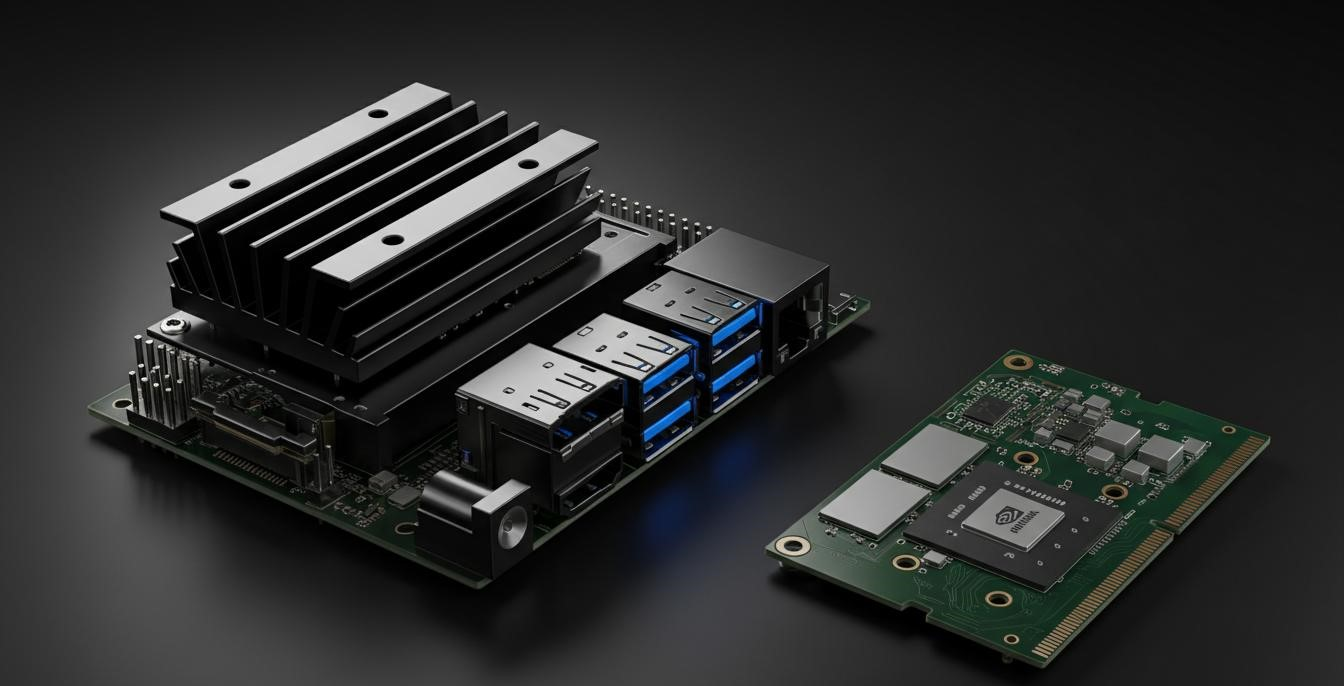
\includegraphics[width=\linewidth]{images/Jetson1}
				\end{tikzfigure}	
			}
			
			\colorlet{blocktitlebgcolor}{blue}
			\block{Project Overview}
			{
				This project demonstrates a \textbf{lightweight, real-time automatic number plate detection system} built on the \textbf{NVIDIA Jetson Nano}. The system is designed for \textbf{edge deployment}, requiring minimal power and computational resources while maintaining efficient performance.
				
				The workflow includes:
				\begin{itemize}
					\item Capturing vehicle footage using a \textbf{camera module}.
					\item Detecting number plates in real-time with \textbf{YOLOv5} for high-speed object detection.
					\item Extracting alphanumeric text from the detected plates using \textbf{Tesseract OCR}.
					\item Storing or processing the recognized plate data for applications such as \textbf{smart parking}, \textbf{access control}, or \textbf{traffic monitoring}.
				\end{itemize}
				
				Key features:
				\begin{itemize}
					\item \textbf{Real-time detection} with low latency suitable for live monitoring.
					\item \textbf{Compact and efficient hardware} ideal for embedded or mobile applications.
					\item \textbf{Versatile integration} with systems like smart gates, automated parking, and vehicle tracking frameworks.
				\end{itemize}
			}
			
			
			\colorlet{blocktitlebgcolor}{blue}
			\block{EU Number Plate Image}
			{
				\begin{tikzfigure}
					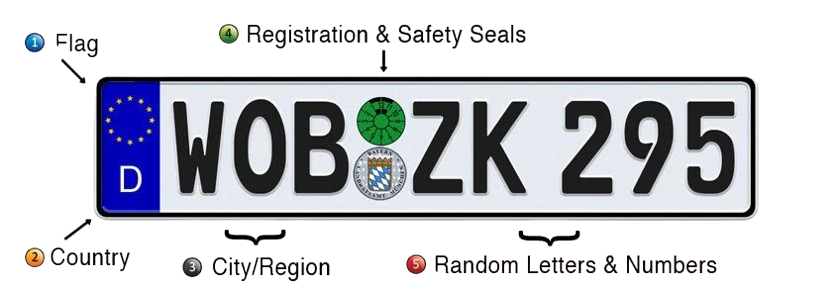
\includegraphics[width=\linewidth]{images/EUplate1}
				\end{tikzfigure}	
			}
			
			\colorlet{blocktitlebgcolor}{blue}
			\block{EU Number Plate Details}
			{
				The \textbf{European Union (EU) number plate format} is standardized for uniformity and easy recognition across member states. Each plate typically features:
				
				\begin{itemize}
					\item A \textbf{blue strip on the left} with the \textbf{EU flag (12 stars)} and \textbf{country code} (e.g., D for Germany, F for France).
					
					\item \textbf{Regional or city codes} showing the registration area (e.g., “B” for Berlin).
					
					\item \textbf{Letters and numbers} forming the unique vehicle identifier, separated by a hyphen or space.
					
					\item An official \textbf{registration seal or hologram} verifying authenticity and authority of issue.
					
					\item A \textbf{standard typeface and spacing} for consistent appearance and accurate OCR detection.
				\end{itemize}
				
				Some plates also use \textbf{special colors or markings}—green for electric, red for temporary, and yellow for export or dealer vehicles.
			}
			
			
			
		
		}
		
		
		\column{0.36}
		{
			\colorlet{blocktitlebgcolor}{blue}
			\block{Hardware Configuration}
			{
				The system utilizes a compact yet powerful set of components optimized for real-time image processing. Each element plays a crucial role in enabling efficient number plate detection and recognition.
				
				\begin{itemize}
					\item \textbf{Jetson Nano (4GB):} Serves as the core processing unit, capable of running AI models locally with CUDA-accelerated inference while maintaining low power consumption.
				
					
					\item \textbf{YOLOv5 Model:} Performs high-speed, accurate object detection to identify and localize number plates in real-time video streams.
					
					\item \textbf{Tesseract OCR Engine:} Extracts alphanumeric text from detected plates, converting them into machine-readable format for logging or verification.
					
					\item \textbf{Display and Monitoring:} Real-time output is displayed through HDMI or accessed remotely via a connected dashboard for system monitoring and testing.
				\end{itemize}
				
				Together, these components form a lightweight yet capable embedded vision system.
			}
			
		
			\colorlet{blocktitlebgcolor}{blue}
			\block{Camera and Sensor Rendering}
			{
				\begin{tikzfigure}
					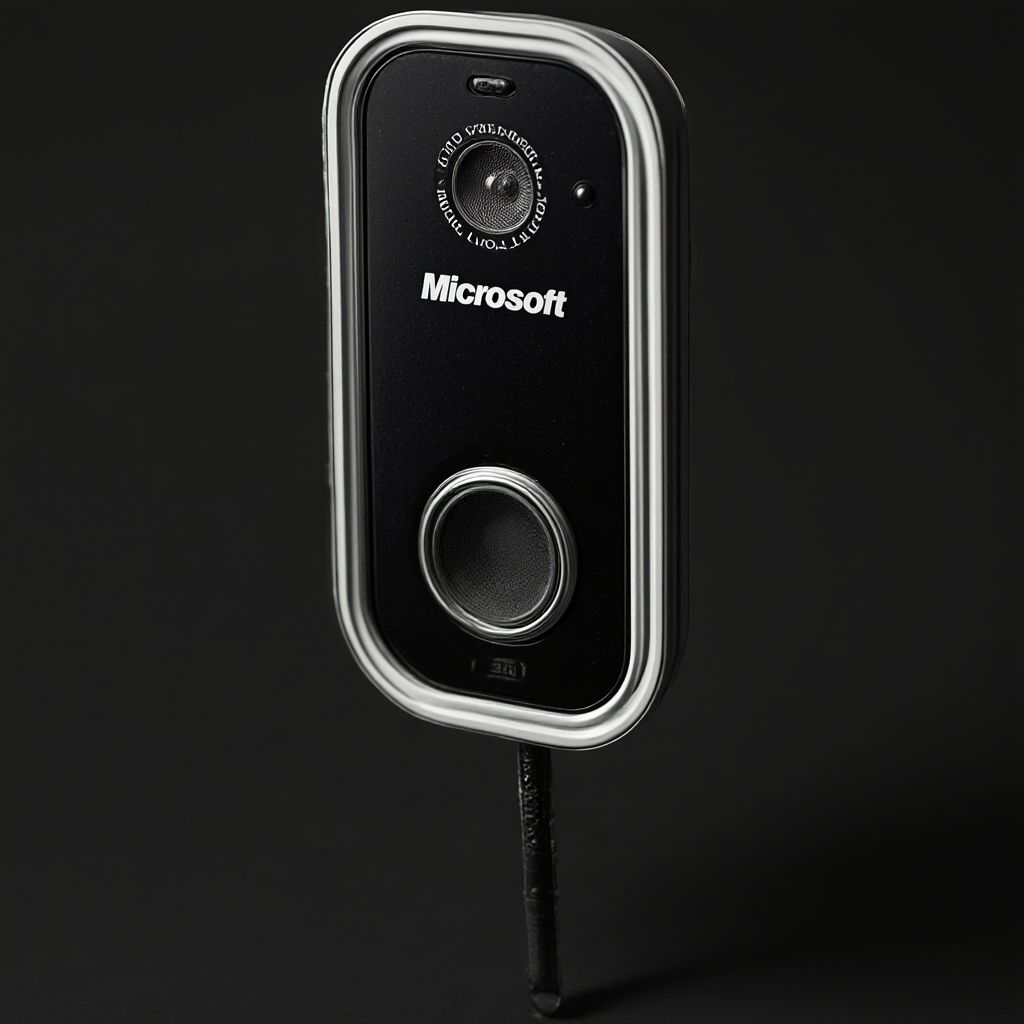
\includegraphics[width=\linewidth]{images/Sensor Camera Rendered}
				\end{tikzfigure}
			}
			
		
				
			\colorlet{blocktitlebgcolor}{blue}
			\block{Future Scope}
			{
				The current system demonstrates effective real-time detection and recognition, but there is significant potential for further development and deployment enhancements. Future improvements include:
				
				\begin{itemize}
					\item \textbf{Enhanced Image Robustness:} Improve detection accuracy under challenging conditions such as motion blur, rain, fog, and low-light environments using image enhancement and data augmentation techniques.
					
					\item \textbf{Region-Specific OCR Training:} Fine-tune the OCR model to better recognize diverse and localized number plate formats across different countries or regions.
					
					\item \textbf{Data Logging and Analytics:} Implement automatic storage of recognized plate data in a local or cloud-based database for record-keeping, analytics, and system monitoring.
					
					\item \textbf{Integration with Smart Infrastructure:} Connect the system with automated gates, barriers, or toll systems to enable fully automated access control or smart parking management.
					
					\item \textbf{Scalability and Deployment:} Optimize the model for deployment on multiple Jetson devices or integrate with IoT frameworks for large-scale, distributed vehicle monitoring networks.
					
					\item \textbf{Real-Time Alerts and Security:} Add features for instant notifications or alerts in case of unauthorized or flagged vehicles.
				\end{itemize}
			}
			
		
		}
	\end{columns}
	
\end{document}
